\documentclass[a4paper,12pt]{article}
\usepackage[margin=2cm]{geometry}

% Pacchetti utili di base
\usepackage[utf8]{inputenc}   % codifica dei caratteri
\usepackage[T1]{fontenc}      % font encoding
\usepackage[italian]{babel}   % lingua italiana
\usepackage{graphicx}         % immagini
\usepackage{hyperref}         % link cliccabili
\usepackage{amsmath}          % align center
\usepackage{listings}         %codice programmazione
\usepackage{xcolor}           % per colori opzionali del codice

% Informazioni sul documento
\title{Tecnologie Web}
\author{Nicolò Giuliani}
\date{}

\lstset{
  language=HTML,
  basicstyle=\ttfamily\small,
  keywordstyle=\color{blue},
  stringstyle=\color{red},
  commentstyle=\color{gray},
  breaklines=true
}

\begin{document}
\maketitle
\tableofcontents   % <-- genera automaticamente la pagina dell'indice
\newpage 

\section{I set di caratteri}
Internet ha proposto il problema di rendere correttamente gli alfabeti di migliaia di lingue nel mondo. Bisogna utilizzare una rappresentazione digitale del testo, ovvero identificare gli elementi e lo spazio. Poi lo definiamo come standard.
\begin{itemize}
  \item caratteri: accenti, maiuscolo/minuscolo, segni aggiuntivi, ecc...
  \item spazio: \\
  - ordine: alfabetico \\
  - contiguità: ogni valore numerico è associato ad un carattere \\
  - raggrupamento: a seconda del valore numerico si definiscono dei gruppi logici
\end{itemize}
A seconda del sistema numerale (bit / hexa) la matematica non cambia rimane invariata.
bbbbbbbbbbbbbbbb
Questo perchè c'è una connessione diretta tra rappresentazione binaria e esadecimale dei numeri secondo cui ogni blocco di 4 cifre binarie (bit) corrisponde ad una cifra esadecimale. 
\begin{align*}
  1bit = 2^1 \text{ combinazioni}: 2 \text{ valori} \\
  2bit = 2^2 \text{ combinazioni}: 4 \text{ valori} \\
  4bit = 2^4 \text{ combinazioni}: 16 \text{ valori} \\
  8bit = 2^8 \text{ combinazioni}: 256 \text{ valori} \\
  16bit = 2^{16} \text{ combinazioni}: 65536 \text{ valori}
\end{align*}
\begin{itemize}
  \item \textbf{ASCII} definisce 128 caratteri (7bit), di cui 33 di controllo (NUL, ESC, TAB, ecc.), con ripetizioni, e 95 caratteri di alfabeto latino, maiuscole, minuscole, numeri, punteggiatura, ecc. 
  \item EBCDIC (contemporaneo ad ASCII), creato dalla IBM per i mainframe, utilizza 8bit con 56 codici di controllo e le lettere dell'alfabeto NON sono continue.
  \item ISO 646-1991 sistema europeo dove si lasciavano 12 codici liberi per nazione per i propi fini, si sacrificavano questi caratteri "\$ @ \ ¬ ` { | } ~".
  \item Code page per ASCII: vari ampliamenti del vecchio standard per amplicare da 128 a 255, però non c'è modo se non esterno di capire quale code page è stata utilizzata.
  \item ISO 8859/1 (ISO Latin 1): una nuova sequenza basata su ASCII per i primi 128 caratteri ma che venivano ampliati a 256.
  \item \textbf{Unicode} e ISO/IEC 10646: due standard internazionali che si sono poi uniti (nel 2020) con gli stessi codici con codifiche a lunghezza variabile (UTF-8, UTF-16, ecc) e fissa (UCS-2, UCS-4). Nel 2025 si definiscono 160k caratteri. \\
  - Unicode include tutti i caratteri degli alfabeti in ordine originale, molto efficiente, caratteri semplici (no bold). Quando possibile due caratteri comuni vengono unificati, sistema perfettamente stabile (quando un carattere viene definito non vengono modificato) e per convertirli in altri formati è molto semplice.  \\
  - UCS-2 è uno schema a piani di 2byte, mentre UCS-4 lo estende ed è uno schema di 31bit in 4byte. \\
  \begin{figure}[h] % [h] = qui (here)
    \centering
    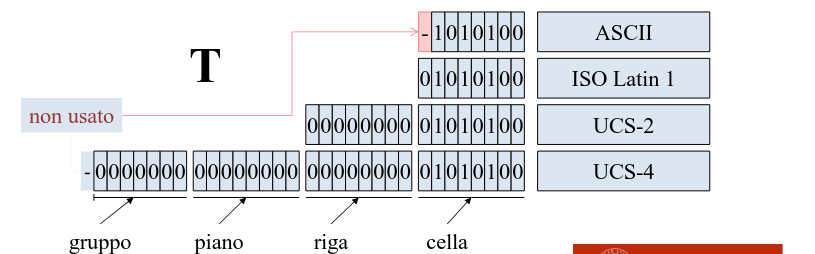
\includegraphics[width=0.7\textwidth]{img/ucs.png}
\end{figure} \\
I piani sono definiti cosi:
\begin{itemize}
  \item Piano 0 (BMP o Basic Multilingual Plane): alfabeti moderni
  \item Piano 1 (SMP o Supplementary Multilingual Plane): alfabeti antichi
  \item Piano 2 (SIP o Supplementary Ideographic Plane): ulteriori caratteri ideografici CJK (Chinese, Japanese, Korean) non presenti in BMP.
  \item Piano 3 (TIP o Tertiary Ideographic Plane): caratteri cinesi antichi
  \item Piano 4-13 sono riservati o inutilizzati 
  \item Piano 14 (SSP o Supplementary Special-purpose Plane): Caratteri tag, in disuso
  \item Piani 15 e 16: Private Use Areas
\end{itemize}
\end{itemize}
Dato che utilizzare 4byte per carattere come in UCS è esagerato nella maggior parte dei casi si utilizza UTF, ovvero un sistema di lunghezza variabile. 
\begin{itemize}
  \item UTF-16: utilizzando 2048 valori a coppie surogate con sequenze a 32bit ci permette di avere un code point dei piani 1-16.
  \item UTF-8: accede ad tutti i caratteri di UCS-4 ma con un numero variabile tra 1 e 4 byte.
\end{itemize}
\vspace{1em}
Come posso capire se il sistema che utilizzo sia little-endian o big-endian (primo byte significativo)? Attraverso il Byte Order Mark (BOM) si aggiunge ovunque (non in mezzo) il carattere $FEFF$ e si capisce che è big-endian, in caso opposto little-endian. \\
Tra UTF-8 e Latin 1 non ci sono differenze per i caratteri ASCII ma per le lettere speciali (accenti, ecc.) cambia, infatti UTF-8 utilizza 2byte mentre Latin 1 solanto 1byte. \\
\begin{figure}[h] % [h] = qui (here)
    \centering
    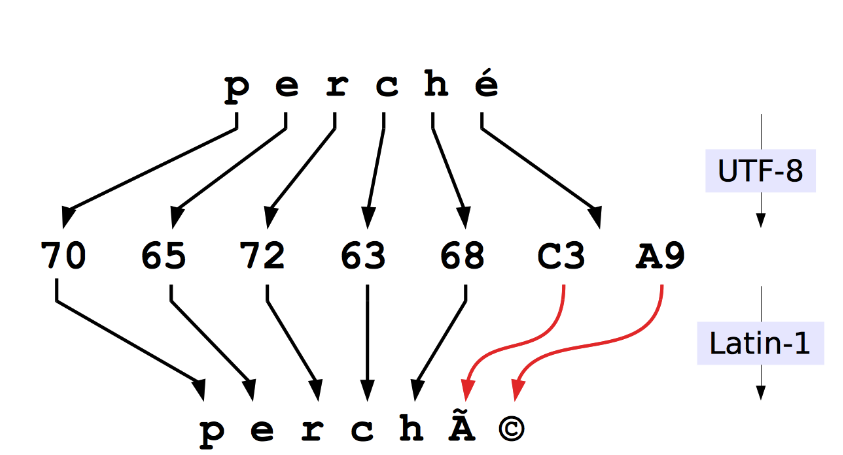
\includegraphics[width=0.5\textwidth]{img/utf-latin.png}
\end{figure} \\
\vspace {5em}
\section{Markup}
\subsection*{Strutture di dati} 
Come abbiamo studiato in precedenza esistono vari modi per organizzare i dati
\begin{itemize}
  \item Record (tupla)
  \item Liste 
  \item Tabelle
  \item Alberi 
  \item Grafi 
\end{itemize}
\subsection{Formati per strutture di dati}
Vediamo che formati possiamo trovare
\begin{itemize}
  \item Tabelle \\
  - CSV: vecchio formato per i dati tabulari, la prima riga è il nome di un campo, una riga è definita dal ritorno a capo, il separatore di campo è dato da virgola, punto, barra verticale, ecc. \\
  - Exel / Libre office: XLSX è il formato di Microsoft  
  \item Alberi \\
  - json: nativo per javascript, supporto su tutti i linguaggi, le parentesi graffe/quadre indicano i contenitori \\
  - yaml: basato come struttura di json ma influenzato da python
  \item Grafi \\
  - RDF: è un modello concettuale, utilizza URI, le informazioni possono essere raggrupate per soggetto 
  \item Testo \\
  - plain text \\
  - Tex / LaTeX \\
  - Html: attuale base del web basato su tag, utilizza anche altri linguaggi come CSS e javascript \\
  - XML: come per html si utilizzano i tag, enfasi sul markup descrittivo e gerarchie\\
  - Markdown
\end{itemize}
\paragraph{Cosa è il markup? \\} 
E' una qualsiasi forma di interpretazione del testo \\
\begin{figure}[h] % [h] = qui (here)
    \centering
    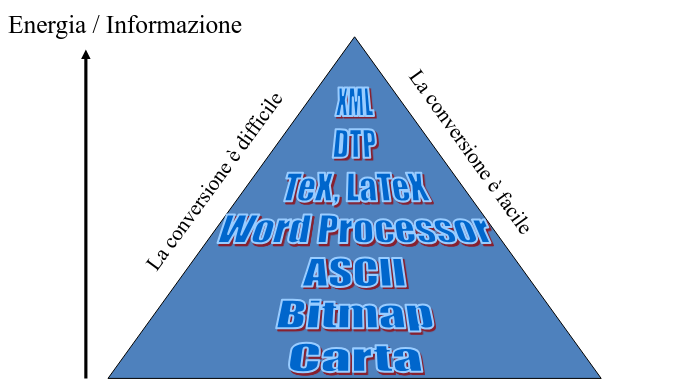
\includegraphics[width=0.5\textwidth]{img/markup.png}
\end{figure} \\
Bisogna per prima cosa definire che esistono sia modi pubblici che privati, ovviamente il secondo caso è quando una azienda ne detiene i diritti per scopi commerciali quindi può modificarlo, aggiornalo per qualsiasi motivo. \\
Esistono anche la distinzione fra binario e visibile, nel secondo caso un essere umano può modificarlo manualmente attraverso un formato leggibile, mentre nel primo caso il testo non è visibile. \\
Definiamo anche interno o esterno quando le istruzioni di presentazione sono in mezzo le parole o se separati in due blocchi di informazioni.
\begin{itemize}
  \item Markup puntuazionale: consiste nell’usare un insieme prefissato di segni per fornire informazioni perlopiù sintattiche sul testo
  \item Markup presentazionale: l markup presentazionale consiste nell’indicare effetti (tipografici o altro) per rendere più chiara la presentazione del contenuto. Attraverso cambi di paragrafo o di pagina, interlinea, pallini per liste, ecc
  \item Markup procedurale: consiste nell’indicare con precisione ad un sistema automatico che effetto attivare e che procedura (serie di istruzioni) eseguire nella visualizzazione del contenuto.
  \item Markup descrittivo: consiste nell’identificare strutturalmente il tipo di ogni elemento del contenuto. Per esempio definendo se si tratta di un titolo, paragrafo, citazione, ecc.
  \item Markup referenziale: consiste nel fare riferimento ad entità esterne al documento per fornire significato o effetto grafico ad elementi del documento. (Es. "CdL"!diventa "Corso di Laurea")
  \item Metamarkup: regole di interpretazione del markup e permette di estendere o controllare il significato del markup
  \item Markup metabolizzato: maiuscole/minuscole, punteggiatura, spazi e ritorni a capo sono essi stessi elementi di markup
\end{itemize}
\subsection{Linguaggi di markup}
\begin{itemize}
  \item TROFF/NROFF: utilizzato oggi giorno per la documentazione tecnica, comandi esterni/interni, definisce 4 tipi di carattere come "roman, italic, bold, symbol". 
  \item Tex / LaTeX: generazione di macro che semplificano notevolmente la generazione di testi particolarmente sofisticati. Attraverso le librerie si semplifica molto gli argomenti complessi.
  \item Linguaggi wiki: usato per documentazione e knowledge base; adatto a non programmatori. Utilizzato da Wikipedia. 
  \item Markdown: orientato alla leggibilità in testo puro, set ristretto di costrutti: titoli, enfasi, link, elenchi, code span, blocchi di codice, molto estendibile ed diffuso. Utilizzato ovunque (README, note, blog, ecc)
  \item json: ottimo per API e storage, non per il testo
  \item yaml: ottimo per file di configurazione e manifest
  \item SGML: un meta-linguaggio (standard) non proprietario di markup descrittivo
\end{itemize}
Un meta-linguaggio è un linguaggio per definire linguaggi, una grammatica di costruzione di linguaggi. Quindi SGML non è un linguaggio di markup, ma un linguaggio con cui definiamo linguaggi di markup. \\
Un documento in un linguaggio di markup definito sulla base di SGML è sempre composto delle seguenti tre parti
\begin{itemize}
  \item Dichiarazione SGML (non obbligatorio) \\
  - Essa permette di specificare valori fondamentali come la lunghezza dei nomi degli elementi, il set di caratteri usati, le specifiche caratteristiche di minimizzazione ammesse, ecc.)
  \item Dichiarazione di documento (DOCTYPE) \\
  - Vengono cioè elencati [i file che contengono] gli elementi ammissibili, il contesto in cui possono apparire, ed altri eventuali vincoli strutturali
  \item Istanza del documento \\
  - L’istanza del documento è quella parte del documento che contiene il testo vero e proprio, dotato del markup appropriato. Esso contiene una collezione di elementi (tag), attributi, entità, PCDATA, commenti, ecc.
\end{itemize}
Un document di markup derivato da SGML (HTML, XML, ecc.) hi i seguenti elementi
\begin{itemize}
  \item Elementi \\ 
  - Un elemento è individuato da un tag iniziale, un contenuto ed un tag finale. Non confondere elemento con TAG!
  \item Attributi \\
  - Gli attributi sono informazioni aggiuntive sull’elemento che non fanno effettivamente parte del contenut
  \item Entità \\
  - Le entità sono frammenti di documento memorizzati separatamente e richiamabili all’interno del documento. Esse permettono di riutilizzare lo stesso frammento in molte posizioni 
  \item Testo 
  \item Commenti \\
  - Sono molto comodi per passare informazioni tra un autore e l’altro, o per trattenere informazioni per se stessi, nel caso le dimenticassimo.
  \item Processing instructions \\
  - sono elementi particolari (spesso di senso esplicitamente procedurale) posti dall’autore o dall’applicazione per dare ulteriori indicazioni su come gestire il documento XML nel caso specifico
\end{itemize}
XML 1.0 (1998) è definito come un sottoinsieme di SGML. XML permette di avere documenti senza l'obbligo di tutti i tag, elementi vuoti, entità definite, ecc. rispetto ad SGML.
\section{HTML}
Html nasce come linguaggio di markup per documenti ipertestuali e multimediali. Ora vediamo la struttura di un documento html:
\begin{lstlisting}
<!DOCTYPE html>
<html>
  <head>
    <title>Document title</title>
  </head>
  <body>
    <p>Text of a paragraph</p>
  </body>
</html>
\end{lstlisting}
analizziamo gli elementi fondamentali
\begin{itemize}
  \item <!DOCTYPE html>: segnala il tipo di markup usato nel documento e la sua versione, con molte complessità e variazioni
  \item html: La radice dell'albero
  \item head: Informazioni globali sul documento. TAG:
  \begin{itemize}
    \item <title>: il titolo del documento
    \item <link>: link di documenti a tutto il documento
    \item <script>: librerie di script
    \item <style>: librerie di stili
    \item <meta>: meta-informazioni sul documento
    \item <base>: l’URL da usare come base per gli URL relativi
  \end{itemize}
  \item body: Il contenuto del documento
\end{itemize}
\subsection*{Elementi inline}
Si dividono in elementi fontstyle e elementi phrase. Molti sono deprecati, e si suggerisce comunque sempre di usare gli stili CSS.
\begin{itemize}
  \item TT (TeleType, font monospaziato, ad es. Courier)
  \item I (corsivo)
  \item B grassetto
  \item U (sottolineato - deprecato)
  \item S e STRIKE (testo barrato - deprecato)
  \item BIG, SMALL (testo più grande e più piccolo)
\end{itemize}
\subsection*{Elementi di blocco}
I tag di blocco definiscono l’esistenza di blocchi di testo che contengono elementi inline
\begin{itemize}
  \item <p>: paragrafo
  \item <div>: Blocco generico
  \item <pre>: blocco preformattato
  \item <address>: l'autore della pagina
  \item <blockquote>: Citazione lunga
\end{itemize}
Blocchi con ruolo strutturale
\begin{itemize}
  \item <h1>, <h2>, <h3>, <h4>, <h5>, <h6>: header
\end{itemize}
\subsection*{Elementi di lista}
Le liste sono contenitori di elementi omogenei
\begin{itemize}
  \item <ul>: Unordered list: lista non ordinata di elementi <li> \\
  - Attributi: type (disc, square, circle)
  \item <ol>: ordered list: lista ordinata di elementi <li> \\
  - Attributi: start (valore iniziale) e type (1, a, A, i, I)
  \item <dl>: lista di definizioni, composta di molti elementi <dt> (definition term) e <dd> (definition data) 
\end{itemize}
\subsection*{Elementi generici}
Sono elementi privi di caratteristiche semantiche o presentazionali predefinite, assumono quelle desiderate con l’aiuto dei loro attributi (style, class, lang).
\begin{itemize}
  \item <div> mantiene la natura di elemento blocco, il resto è neutro
  \item <span> mantiene la natura di elemento inline, il resto è neutro
\end{itemize}
\subsection*{Effetti grafici minori}
\begin{itemize}
  \item <hr> (horizontal rule): una piccola riga orizzontale attraverso lo schermo. Si può controllarne la larghezza e lo spessore
  \item <br> (break): una andata a capo forzata (non spezza logicamente il paragrafo, impone semplicemente il cambio riga)
\end{itemize}
\subsection*{Elementi di struttura}
HTML 5 introduce nuovi elementi con una semantica precisa, per organizzare il documento in contenitori che possono essere più facilmente manipolati, esportati, modificati, etc.
\begin{itemize}
  \item <main>: la parte principale della pagina, ovvero un contenitore di testo o di sottosezioni che rappresenta la parte più importante della pagina. Al suo interno possiamo trovare: 
  \begin{itemize}
    \item <section>: un contenitore generico annidabile
    \item <article>: una parte del documento self-contained e pensata per essere ri-usata e distribuita come unità atomica (post di un blog, news, feed, etc.)
  \end{itemize}
  \item <aside>: una sezione collegata al testo ma separata dal flusso principale (note a margine, sidebar, incisi, pubblicità, etc.)
  \item <header>: contiene l’intestazione della sezione corrente o dell’intera pagina ed è solitamente usato per tabelle di contenuti, indici, form di ricerca, intestazioni
  \item <footer>: contiene la "parte conclusiva" della sezione corrente o dell’intera pagina. E’ usato principalmente per mostrare informazioni (testuali, non metadati) sugli autori della pagina, copyright, produzione, licenze
  \item <nav>: liste di navigazione, sono molto utili per l’accessibilità, in quanto possono essere più facilmente identificate e accedute anche da utenti disabili (tramite screenreaders o altri ausili)
\end{itemize}
\subsection*{Link}
I link sono definiti con elementi <a> (àncore nel documento, elemento inline), attributi:
\begin{itemize}
  \item href: specifica l'URL della destinazione
  \item name: specifica un nome che può essere usato come ancora di destinazione di un link (non si vede che il testo è blu com eun link, rimane nero)
\end{itemize}
\subsection*{Immagini}
Le immagini inline sono definite con l'elemento <img>. Formati tipici: jpeg, gif, png.
\begin{itemize}
  \item <img> è un elemento vuoto, completamente definito dai suoi attributi. \\
  \begin{itemize}
    \item src (required): l'URL della risorsa contenente l'immagine
    \item alt: testo alternativo se l'immagine non è mostrata
    \item width: forza una larghezza in pixel per l'immagine.
    \item height: forza una altezza in pixel per l'immagine
  \end{itemize}
\end{itemize}
Attraverso l'attributo srcset è possibile indicare più risorse per la stessa immagine, da usare alternativamente. A seconda dello user agent scegliamo immagini con dimensioni (e quindi risoluzioni) diverse, e non dobbiamo affidarci al ridimensionamento algoritmico dell'immagine con l'inevitabile perdita di dettaglio
\begin{lstlisting}
<img srcset="kitten-480w.jpg 480w, kitten-1080w.jpg 1080w"
  sizes="(max-width: 800px) 480px, 1080px"
  src="kitten-800w.jpg"
  alt="A pretty kitten">
\end{lstlisting}
\begin{itemize}
  \item L'attributo srcset indica quali risorse usare e la dimensione "reale" di ciascuna risorsa
  \item L'attributo sizes indica quali tipi di schermo associare a ciascuna risorsa
  \item L'attributo src è un fallback nel caso che il browser non conosca srcset
\end{itemize}
\subsection*{L'elemento <figure>}
Le immagini sono dunque elementi vuoti inline. In molte situazioni ho bisogno di un elemento complesso, di tipo blocco, magari con didascalia e marginatura controllabile.
\begin{figure}[h] % [h] = qui (here)
    \centering
    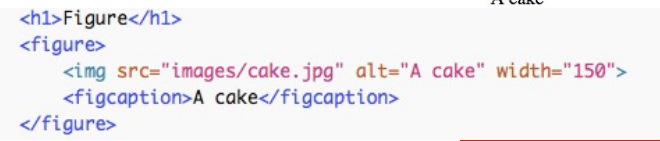
\includegraphics[width=0.7\textwidth]{img/figure.png}
\end{figure}
\subsection*{Embedding}
Permettono di arricchire la pagina HTML con molteplici tipi di contenuti alternativi.
\begin{itemize}
  \item <video> per fare embedding di un video
  \item <audio> per fare embedding di un audio
  \item <object> per fare embedding di oggetti multimediali, vediamo quali:
  \begin{itemize}
    \item <canvas>: possibilità di disegnare direttamente sulla pagina interagire con gli oggetti multimediali
    \item <video>: meccanismo generico per il caricamento di file e stream video. Posisbilità di avere diversi file, tra i quali il browser sceglie quello da eseguire.
    \item <audio>: (uguale a video)
    \item <math>
  \end{itemize}
  \item <embed> elemento generico per fare embedding di oggetti multimediali. Un po' in disuso
  \item <iframe> per fare embedding di una pagina HTML all'interno di un'altra pagina HTML.
\end{itemize}
\begin{lstlisting}
<iframe title="Mappa OpenStreetMap - Bologna Centro"
  width="300" height="200" loading="lazy"
  referrerpolicy="no-referrer"
  sandbox="allow-scripts allow-same-origin"
  src="https://www.openstreetmap.org/export/embed.html?bbox=11.320%2C44.490%2C11.370%2C44.500">
</iframe>
\end{lstlisting}
\subsection*{Tabelle}
Le tabelle vengono specificate riga per riga. Di ogni riga si possono precisare gli elementi, che sono o intestazioni o celle normali. Una tabella può anche avere una didascalia, un’intestazione ed una sezione conclusiva. E’ possibile descrivere insieme le caratteristiche visive delle colonne.
\begin{lstlisting}
<table border="1" >
  <tr>
    <th>Salesman</th><th>Jan</th>
    <th>Feb</th><th>Mar</th>
  </tr>
  <tr>
    <th>John Smith</th> <td>12000</td>
    <td>13000</td><td>15000</td>
  </tr>
</table>
\end{lstlisting}
Possiamo anche definire \textit{rowspan} e \textit{colspan} per allargare le celle
\begin{lstlisting}
<table border="1" >
  <tr>
    <td>First row <br> First collumn</td>
    <td colspan="2">First row <br> Second column</td>
  </tr>
  <tr>
    <td colspan="2">Second row <br> First column</td>
    <td rowspan="2">Secondrow <br> Thrird column</td>
  </tr>
  <tr>
    <td>Third row <br> First column</td>
    <td>Third row <br> Second column</td>
  </tr>
</table>
\end{lstlisting}
\begin{figure}[h] % [h] = qui (here)
    \centering
    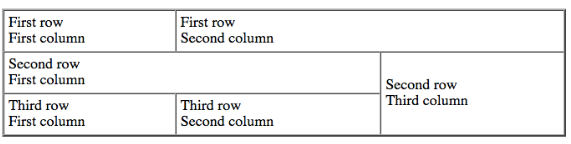
\includegraphics[width=0.7\textwidth]{img/tables.png}
\end{figure}
\subsection*{Form}
Con i FORM si utilizzano le pagine HTML per inserire valori che vengono poi elaborati sul server. I FORM sono legati ad applicazioni server-side.  Crea una connessione HTTP con il server, specificando una ACTION (cioè un applicazione che funga da destinatario) a cui fare arrivare i dati. Il destinatario riceve i dati, li elabora e genera un documento di risposta, che viene spedito, tramite il server HTTP, al browser.
\begin{itemize}
  \item <form>: il contenitore dei widget del form. Attributi:
  \begin{itemize}
    \item method: il metodo HTTP da usare (GET, POST)
    \item action: l'URI dell'applicazione server-side da chiamare
  \end{itemize}
  \item <input>, <select>, <textarea>: i widget del form. Attributi:
  \begin{itemize}
    \item name: il nome del widget usato dall'applicazione server-side per determinare l'identità del dato
    \item type: il tipo di widget (input, checkbox, radio, submit, reset, etc.)
  \end{itemize}
  \item <button>: un bottone cliccabile (diverso dal submit
  \item <label>: la parte visibile del widget
\end{itemize}
HTML LS introduce molte novità per velocizzare, semplificare e controllare l’inserimento dei dati da parte dell’utente. L’oggetto \textit{input} è arricchito con molti attributi che permettono di controllare il focus e aggiungere suggerimenti agli utenti:
\begin{itemize}
  \item placeholder: contiene una stringa che sarà visualizzata in un campo di testo se il focus non è su quel campo
  \item required: il form non può essere sottomesso senza una valore per questo elemento
  \item readonly: è un elemento del form non modificabile
  \item list: il valore deve appartenere ad uno dei valori ammessi (specificati in un elemento <datalist> associato
\end{itemize}
\begin{lstlisting}
<input type="text" list="province">
<datalist id="province">
  <option value="BO">Bologna</option>
  <option value="MO">Modena</option>
  <option value="FC">Forli Cesena</option>
</datalist>
\end{lstlisting}
In HTML LS sono introdotti molti nuovi tipi per l’oggetto input. I browser forniscono widget diversi nell’interfaccia in base al tipo del campo:
\begin{itemize}
  \item email:in fase di validazione il browser verifica se il testo inserito contiene il simbolo '@’ e il dominio è (sintatticamente) corretto
  \item url: si verifica che il testo inserito segue le specifiche degli URL
  \item number: il browser visualizza bottoni per incrementare/decrementare il valore. E’ possibile specificare il valore minimo, massimo e l’unità di modifica in altri attributi di input
  \item range: il browser visualizza uno slider per incrementare o decrementare un valore numerico. E’ possibile specificare il valore minimo, massimo e l’unità di modifica
  \item date: richiede al browser la visualizzazione di un calendario tra cui selezionare una data. Esistono vari tipi collegati come month, week, time (orario), etc.
  \item search: testo renderizzato in modo diverso su alcuni browser (iPhone)
  \item color: usato per mostrare una tavolozza di colori, da cui selezionare un codice RGB
\end{itemize}
\begin{lstlisting}
<p>Nome: <input name="nome" type="text" placeholder="Inserisci qui il tuo nome" size="40" autofocus></p>
<p>Cognome: <input name="cognome" size="40" placeholder="Inserisci qui il tuo cognome"></p>
<p>Email: <input name="mail" type="email"></p>
<p>Lezioni: <input type="number" min="5" max="25" step="1" value="1"></p>
<p>Livello: <input type="range" name="level" min="1" max="10" step="1" value="3"></p>
<p>Data Inizio: <input name="birth" type="date" value="2011-04-01"></p>
<p><input type="submit" value="Iscriviti"></p>
\end{lstlisting}
\subsection{Attributi globali}
Sono attributi globali quelli definiti su tutti gli elementi del linguaggio HTML. Essi costituiscono attributi di qualificazione e associazione globale degli elementi. Per lo più per CSS e link ipertestuali.
\begin{itemize}
  \item Id: un identificativo unico (su tutto il documento)
  \item Class: una lista (separata da spazi) di nomi di classe (per attribuzione semantica e di stile CSS)
  \item Style: un breve stile CSS associato al singolo elemento
  \item Title: un testo secondario associato all’elemento (per accessibilità e informazioni aggiuntive)
\end{itemize}
\begin{figure}[h] % [h] = qui (here)
    \centering
    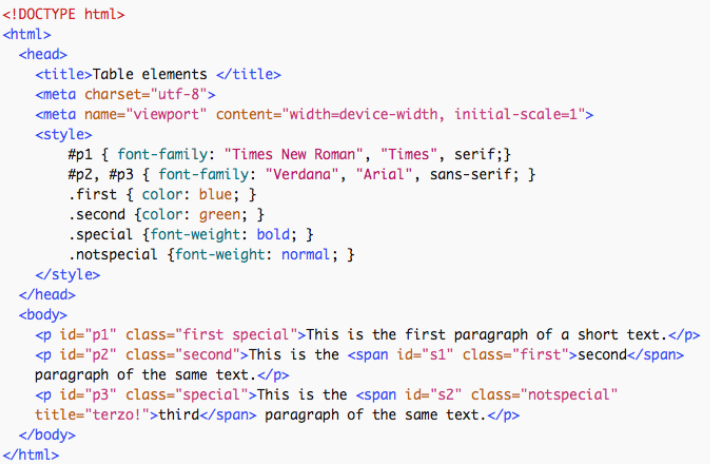
\includegraphics[width=0.7\textwidth]{img/attributi.png}
\end{figure}
\subsection*{Colori}
In molte situazioni (sfondi, caratteri, ecc.) è possibile specificare un colore. HTML fornisce due modi per farlo:
\begin{itemize}
  \item Codice RGB
  \item Nome
\end{itemize}
Tuttavia HTML 4 depreca l’uso esplicito di colori nel documento HTML, e suggerisce di usare i fogli di stile.
\begin{lstlisting}
<font color="#FF0000">testo in rosso</font>
<body bgcolor="#008080">sfondo teal</body>
<td bgcolor="yellow">sfondo giallo</td>
\end{lstlisting}
\subsection*{Lunghezze}
HTML usa le lunghezze per tutti gli oggetti con una presenza sulla pagina di dimensioni determinate (immagini, tabelle, frame, ecc.) Si usano tre tipi di lunghezze:
\begin{itemize}
  \item Pixel: una dimensione in punti di schermo. È un numero assoluto
  \begin{lstlisting}
  <img src="immagine.gif" width="150">
  \end{lstlisting}
  \item Percentuali: una dimensione in proporzione alla dimensione del contenitore. È un numero seguito da un carattere %.
  \begin{lstlisting}
  <table width="100%">...</table>
  \end{lstlisting}
  \item Multi-lunghezze: una sequenza di valori di lunghezza. In questo caso il carattere '*’ divide la quantità restante in parti uguali (dopo aver tolto le lunghezze esplicite in pixel e percentuale).
  \begin{lstlisting}
  <colgroup width="150,25%,*,*">
  \end{lstlisting}
\end{itemize}
\section{CSS}
La \textbf{tipografia} è la disposizione armoniosa di tipi al fine di creare testo leggibile e piacevole alla vista sulla pagina e sugli schermi digitali.
\subsection*{Font e type face}
Un font è una collezione di forme di caratteri integrate armoniosamente per le necessità di un documento in stampa. Tipicamente contiene forme per lettere alfabetiche, numeri, punteggiatura e altre caratteri standard nello scritto. Un type face (o font-family) è uno stile unico di caratteri che viene espanso in molti font di dimensione e peso e stili diversi.
\subsection*{Spazi colori}
L'occhio umano ha tre tipi di coni, celle incaricate di riconoscere colori. Assorbono frequenze diverse della luce riflessa sugli oggetti, che vengono interpretati separatamente dando l'impressioni di colori diversi.
\begin{figure}[h] % [h] = qui (here)
    \centering
    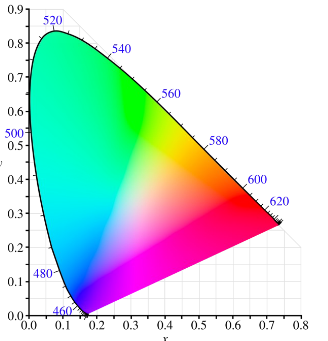
\includegraphics[width=0.15\textwidth]{img/colori.png}
\end{figure} \\
RGB è uno spazio colore additivo basato sull'identificazione di Rosso, Verde e Blu come colori primari. Poiché i coni dell'occhio sono sensibili separatamente alle frequenze del rosso, del verde e del blu, questo è un modello ragionevolmente vicino a quello dell'occhio umano.
\begin{figure}[h] % [h] = qui (here)
    \centering
    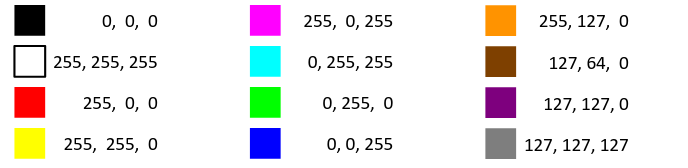
\includegraphics[width=0.4\textwidth]{img/rgb.png}
\end{figure} \\
RGBA è uno spazio colore derivato da RGB, a cui viene aggiunta una quarta dimensione, chiamata canale alpha.
\begin{figure}[h] % [h] = qui (here)
    \centering
    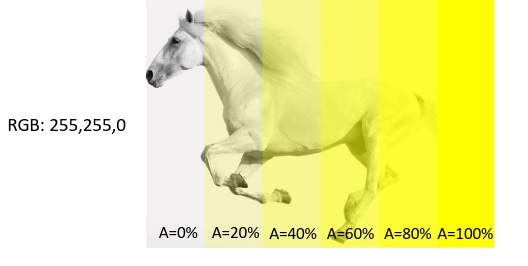
\includegraphics[width=0.4\textwidth]{img/rgba.png}
\end{figure} \\
\subsection*{CMYK}
CMYK è uno spazio colore sottrattivo basato sull'identificazione di quattro colori primari, Cyan, Giallo, Magenta e Key (che è un nero molto scuro).
\begin{figure}[h] % [h] = qui (here)
    \centering
    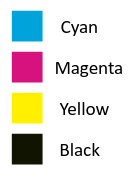
\includegraphics[width=0.1\textwidth]{img/CMYK.png}
\end{figure} \\
Si usa quattro colori invece di tre perché l'inchiostro nero fornisce una definizione dei colori molto migliore, aumentando il contrasto e riducendo la quantità di inchiostro colorato necessario per le tinte più scure.
\subsection{Cascading Style Sheet}
Come si utilizza? In HTML abbiamo
\begin{itemize}
  \item posizionato presso il tag di riferimento
  \begin{lstlisting}
  <html>
    <head>
      <title>Esempio CSS</title>
    </head>
    <body style="background-color:yellow;">
      <h1 class="title" style="color:blue;">
        I CSS: questi sconosciuti
      </h1>
      <p>Un paragrafo senza stile</p>
      <p id="p1" style="color:red;">
        Ecco un primo esempio di uso dei CSS.
      </p>
    </body>
  </html>
  \end{lstlisting}
  \item posizionato nel tag <style>
  \begin{lstlisting}
  <html>
    <head>
      <title>Esempio CSS</title>
      <style type="text/css">
        body { background-color: yellow; }
        p { color: black; }
        .title { color: blue; }
        #p1 { color: red; }
      </style>
    </head>
    <body>
      <h1 class="title">
        I CSS: questi sconosciuti
      </h1>
      <p>Un paragrafo senza stile</p>
      <p id="p1">
        Ecco un primo esempio di uso dei CSS.
      </p>
  </body>
  </html>
  \end{lstlisting}
  \item indicato dal tag <link>
  \begin{figure}[h] % [h] = qui (here)
    \centering
    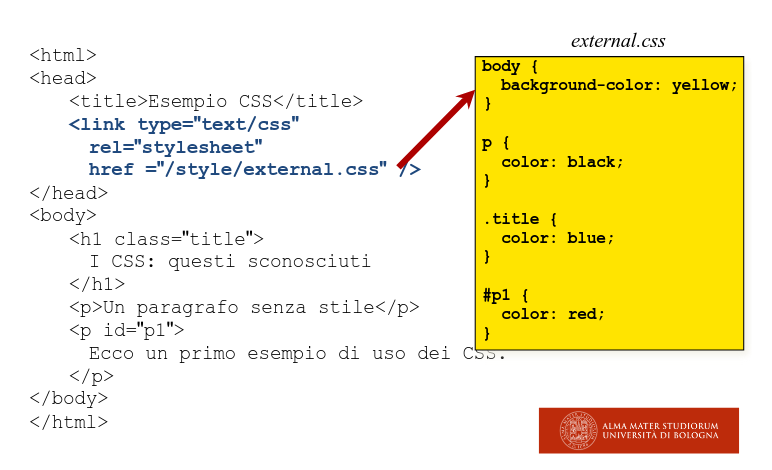
\includegraphics[width=0.7\textwidth]{img/link.png}
\end{figure}
\end{itemize}
Inoltre HTML permette di assegnare gli stili agli elementi in tre modi
\begin{itemize}
  \item assegnati a tutti gli elementi di un certo tipo (il nome dell'elemento)
  \item assegnati a tutti gli elementi di una certa categoria (il valore dell'attributo class)
  \item assegnati ad uno specifico elemento (identificato dal valore dell'attributo id)
\end{itemize}
\subsection{Proprietà}
\paragraph{La scatola\\}
La visualizzazione di un documento con CSS avviene identificando lo spazio di visualizzazione di ciascun elemento.
\begin{itemize}
  \item Margin: la regione che separa una scatola dall'altra, sempre trasparente (ovvero ha il colore di sfondo della scatola contenitore)
  \item Border: la regione ove visualizzare un bordo per la scatola
  \item Padding: la regione di respiro tra il bordo della scatola ed il contenuto. Ha sempre il colore di sfondo del contenuto
  \item Content: la regione dove sta il contenuto dell'elemento
\end{itemize}
  \begin{figure}[h] % [h] = qui (here)
    \centering
    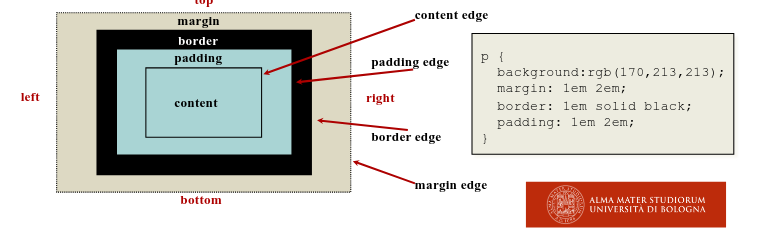
\includegraphics[width=0.8\textwidth]{img/scatola.png}
\end{figure}
\section{Uniform Resource Identifier (URI)}
Attraverso gli URI, il WWW è stato in grado di identificare risorse accessibili tramite il proprio protocollo, HTTP, e tramite tutti gli altri protocolli esistenti. Gli URI (Uniform Resource Identifier) sono una sintassi usata in WWW per definire i nomi e gli indirizzi di oggetti (risorse) su Internet. \\
Gli Uniform Resource Identifier (URI) sono, per definizione:
\begin{itemize}
  \item Locator (URL): una sintassi che contiene informazioni immediatamente utilizzabili per accedere alla risorsa (ad esempio, il suo indirizzo di rete) \\
   \begin{itemize}
      \item Gli URL sono un indirizzo della risorsa che possa essere immediatamente utilizzato da un programma per accedervi.
    \end{itemize}
  \item Names (una volta chiamati URN): una sintassi che permetta una etichettatura permanente e non ripudiabile della risorsa, indipendentemente dal riportare informazioni sull'accesso.
  \begin{itemize}
    \item I names sono un nome stabile e definitivo di una risorsa, che possa fornire un'informazione certa ed affidabile sulla sua esistenza ed accessibilità. \\
    \item I names debbono essere trasformati da un apposito servizio, negli URL attualmente associati alla risorsa. Inoltre la mappa deve essere aggiornata ogni volta che la risorsa viene spostata.
  \end{itemize} 
\end{itemize}
\vspace{3em}  
\begin{figure}[h] % [h] = qui (here)
    \centering
    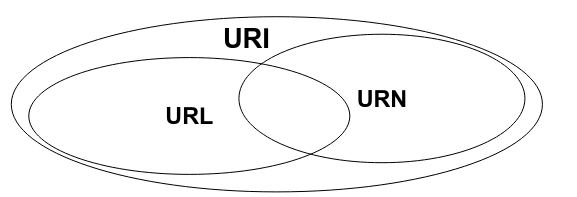
\includegraphics[width=0.7\textwidth]{img/URI.png}
\end{figure}
Nella visione moderna, la distinzione tra locator e name è secondaria rispetto al concetto di schemi: ogni URI appartiene ad uno schema (la parte della stringa che precede i due punti).
\subsection*{Criteri di design degli URI}
Gli URI sono progettati per essere:
\begin{itemize}
  \item Trascrivibili: gli URI sono sequenze di caratteri tratti da un set molto limitato (lettere, numeri, alcuni - pochi - caratteri speciali), per permettere la trascrizione degli URI su canali anche non elettronici (un pezzo di carta, un cartellone, ecc.)
  \item Fornire identificazione, non interazione: le operazioni eseguibili sulle risorse ed i protocolli per eseguirli non sono indicati nell’URI, ma nell’interpretazione che degli URI si fa all’interno dello specifico schema.
  \item Fornire spazi di nomi organizzati gerarchicamente: i caratteri ``:'', ``/'', ``?'' e ``\#'' separano ambiti diversi all’interno degli URI. Il primo, onnipresente ed obbligatorio, è lo schema di interpretazione del resto. Schemi gerarchici usano il carattere ``/'' per separare livelli di specificità diversi del nome locale. ``?'' separa la parte di identificazione della risorsa da qualunque parametro necessario per accedervi, e ``\#'' separa l’identificativo della risorsa da quello del frammento interno a cui si fa riferimento.
\end{itemize}
\begin{center}
URI = schema : [// authority] path [? query] [\# fragment]
\end{center}
Analizziamo nel dettaglio
\begin{itemize}
  \item Schema: protocollo TCP utilizzato
  \item La presenza esplicita di un’authority individua un’organizzazione gerarchica dello spazio dei nomi a cui sono delegati i nomi (che possono essere ulteriormente delegati)
  \begin{itemize}
    \item authority = [userinfo @] host [: port]
  \end{itemize}
  \item La parte path è la parte identificativa della risorsa all’interno dello spazio di nomi identificato dallo schema e (se esistente) dalla authority.
  \item La parte query individua un’ulteriore specificazione della risorsa all’interno dello spazio di nomi identificato dallo schema e dall’URI precedente. Di solito questi sono parametri passati all’URI (un processo) per specificare un risultato dinamico
  \item La parte fragment individua una risorsa secondaria (una risorsa associata, dipendente o in molti casi un frammento) della risorsa primaria.
\end{itemize}
\subsection*{Route}
Una route è un'associazione della parte path di un URI ad una risorsa gestita o restituita da un server web.
\begin{itemize}
  \item Managed route: il server associa ogni URI ad una risorsa o attraverso il file system locale (risorse statiche) oppure generate attraverso una computazione (risorse dinamiche)
  \begin{figure}[h] % [h] = qui (here)
    \centering
    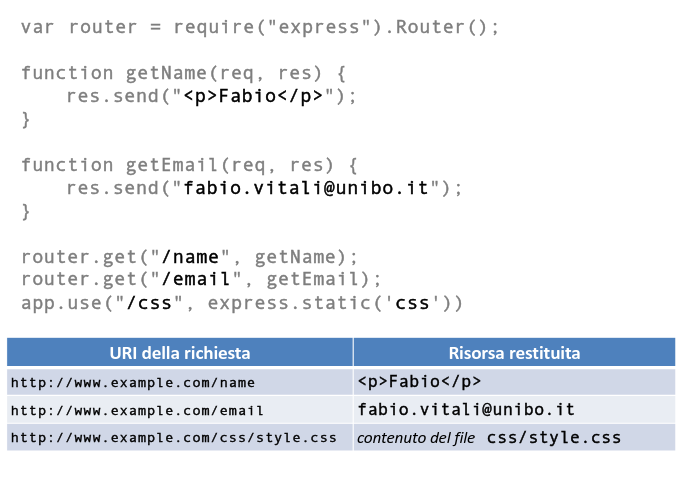
\includegraphics[width=0.7\textwidth]{img/managed.png}
\end{figure}
  \item File-system route: il server associa la radice della parte path ad una directory del file system locale e ogni filename validoall'interno di quella directory genera un URI corretto e funzionante.
  \begin{figure}[h] % [h] = qui (here)
    \centering
    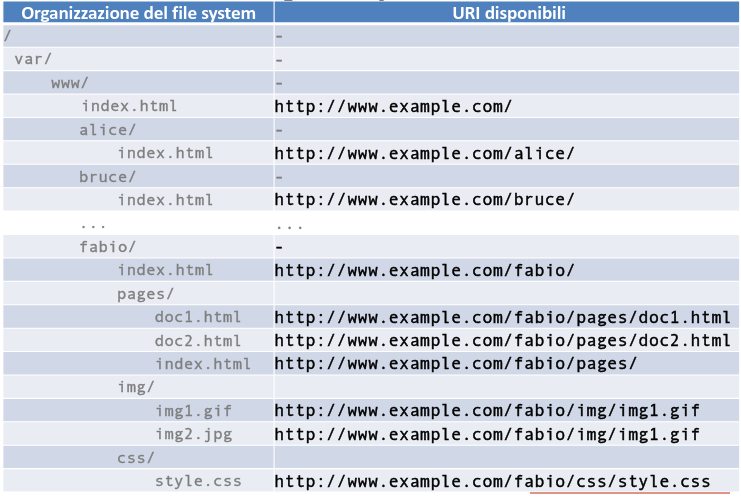
\includegraphics[width=0.7\textwidth]{img/unmanaged.png}
\end{figure}
\end{itemize}
\subsection*{Uri references (uriref)}
Un URI assoluto contiene tutte le parti predefinite dal suo schema, esplicitamente precisate. Un URI reference fa sempre riferimento ad un URI di base (ad esempio, l'URI assoluto del documento ospitante l'URI reference) rispetto al quale fornisce porzioni differenti.
\subsection*{HTTP e HTTPS}
I protocolli più usati nel WWW. HTTPS prevede una crittografazione in entrambi i sensi del contenuto del messaggio.
\subsection*{FILE}
Dà accesso ai file di un file system locale (cioè del computer su cui gira il browser)
\begin{center}
file://host/path [\#fragment]
\end{center}
MS Windows accetta anche "$\backslash$", che però non è nello standard approvato!
\subsection*{DATA}
Uno schema non gerarchico, che non fa riferimento ad una risorsa, ma CONTIENE la risorsa: tutti i dati della risorsa sono inseriti nell'URI vero e proprio. 
\begin{center}
data:[<media type>][;base64],<data>
\end{center}
Si può codificare il dato, di solito usando base64;
\subsection*{FTP}
\begin{center}
ftp://[user[:password]@]host[:port]/path
\end{center}
\subsection*{Content Delivery Network (CDN)}
In breve, una rete fortemente distribuita di server commerciali che collaborano tra loro per distribuire in maniera omogenea contenuti di grande successo senza inutili duplicazioni di occupazione e trasmissione di file. \\
Ad esempio ogni utente che naviga su molti siti web, che usano le stesse librerie importanti ma non le prendono da un CDN, devescaricare tutte le volte gli stessi identici file. Se questi siti invece fanno riferimento a librerie sullo stesso CDN, esse verranno scaricate una volta sola e rimarranno in cache anche per gli altri siti.
\subsection*{IRI}
Internationalized Resource Identifier, RFC 3987 di Gennaio 2005, fornisce una sintassi per inserire caratteri di UCS-4 in un URI e per risolverli. In realtà non tutti i caratteri sono ammessi: tutti i codici di controllo e tutti i codici non corrispondenti a caratteri usati nelle lingue non sono ammessi.
\subsection*{IDN}
Internazionalized Domain Name (IDN), o anche Internazionalized Domain Name for Application (IDNA), è uno standard IETF per estendere i nomi di dominio a tutti i caratteri non ASCII di Unicode (RFC 5890). Questi nuovi nomi di dominio vengono detti IDN.
  \vspace{10em}
  \begin{figure}[h] % [h] = qui (here)
    \centering
    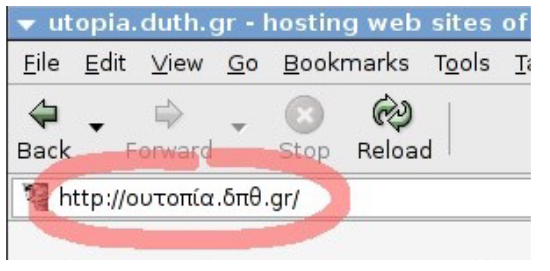
\includegraphics[width=0.5\textwidth]{img/idn.png}
\end{figure} \\
\subsection*{CURIE}
I Compact URI sono un modo per esprimere in maniera compatta famiglie di URI che condividono lo stesso prefisso
\begin{center}
  [prefix:curie]
\end{center}
Il prefisso è associato (in uno di molti modi, ad esempio XML namespaces che vedremo) ad un URI assoluto che deve essere sostituito nel CURIE per ottenere l'URI cercato
\begin{lstlisting}
<html xmlns:dom="http://www.dominio.com/">
  <p>Si veda <a href="[dom:doc1]">doc 1</a></p>
</html>
\end{lstlisting}
In questo caso, il CURIE [dom:doc1] viene risolto nell'URI http://www.dominio.com/doc1
\subsection*{Linked Data}
Il nome Linked Data è stato proposto da Tim Berners-Lee nel 2009 come modello concettuale per la caratterizzazione di tutte le risorse di dati che possono essere messi a disposizione ed incrociati da applicazioni ed umani.
Per essere Linked Data, una collezione di dati deve:
\begin{itemize}
  \item Usare URI per identificare oggetti.
  \item Usare HTTP URI in modo che questi oggetti possano essere referenziati e cercati da persone e user agent.
  \item Fornire informazioni utili sull'oggetto quando la sua URI è dereferenziata, usando formati standard come RDF.
  \item Includere link ad altre URI relative ai dati esposti per migliorare la ricerca di altre informazioni relative nel Web.
\end{itemize}
\section{HyperText Transfer Protocol}
HTTP é un protocollo client-server, generico e stateless utilizzato non solo per lo scambio di documenti Web ma in molte applicazioni distribuite. \\
Una connessione HTTP è composta da una serie di richieste ed una serie corrispondente di risposte:
\begin{itemize}
  \item Pipelining: trasmissione di più richieste senza attendere l'arrivo della risposta alle richieste precedenti. MA le risposte sono restituite nello stesso ordine delle richieste
  \item Multiplexing: nella stessa connessione è possibile avere richieste e risposte multiple, restituite anche in ordine diverso rispetto alle richieste e "ricostruite" nel client
\end{itemize}
HTTP/2 ha introdotto molte novità per migliorare le performance, tra cui:
\begin{itemize}
  \item PUSH: il server anticipa le richieste successive del client
  \item Compressione degli header: i dati non sono trasmessi in chiaro ma compressi (e in parallelo)
\end{itemize}
  \begin{figure}[h] % [h] = qui (here)
    \centering
    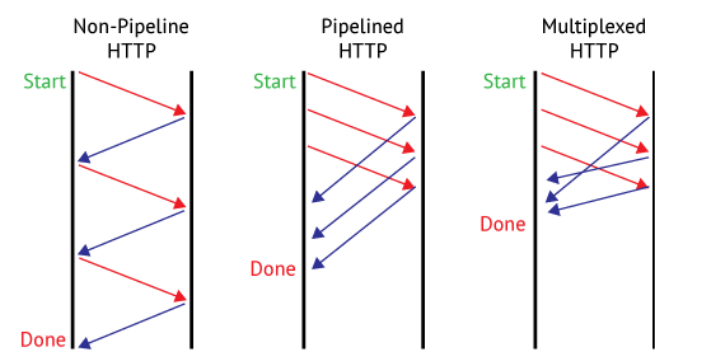
\includegraphics[width=0.7\textwidth]{img/http.png}
\end{figure}
\subsection*{La richesta HTTP}
La richiesta HTTP si compone di:
\begin{itemize}
  \item Method: azione del server richiesta dal client
  \item URI: identificativo della risorsa locale al server
  \item Version: numero di versione di HTTP
  \item Header: sono linee RFC822 divise in header generali, header di entità e header di richiesta
  \item Body: un messaggio MIME
\end{itemize}
  \begin{figure}[h] % [h] = qui (here)
    \centering
    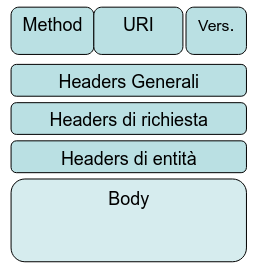
\includegraphics[width=0.3\textwidth]{img/richiesta.png}
\end{figure}
Un esempio di richiesta
\begin{verbatim}
GET /beta.html HTTP/1.1

Referer: http://www.alpha.com/alpha.html
Connection: Keep-Alive
User-Agent: Mozilla/4.61 (Macintosh; I; PPC)
Host: www.alpha.com:80
Accept: image/gif, image/jpeg, image/png, */*
Accept-Encoding: gzip
Accept-Language: en
Accept-Charset: iso-8859-1,*,utf-8
\end{verbatim}
\subsection{I metodi di HTTP}
\begin{itemize}
  \item GET: metodo più frequente (sicuro ed idempotente), ed è quello che viene attivato facendo click su un link ipertestuale di un documento HTML, o specificando un URL nell’apposito campo di un browser per richiede una risorsa ad un server
  \item HEAD: simile (sicuro ed idempotente) al metodo GET, ma il server deve rispondere soltanto con gli header relativi, senza il corpo. Viene usato per verificare validità, accessibilità e coerenza in cache di un URI
  \item POST: serve per trasmettere informazioni dal client al server relative alla risorsa identificata nell'URI (spedire i dati di un form HTML)
  \item PUT: trasmettere delle informazioni (idempotente) dal client al server, creando o sostituendo la risorsa specificata. L’argomento del metodo PUT è la risorsa che ci si aspetta di ottenere facendo un GET in seguito con lo stesso nome
  \item DELETE: rimuovere le informazioni (idempotente e NON sicuro) connesse con una risorsa
  \item PATCH: aggiornare parzialmente (NON idempotente NON sicuro) la risorsa identificata dall'URI.  Usato per indicare quindi modifiche incrementali e non sovrascrivere risorse al server, come ad esempio nel caso di PUT
  \item OPTIONS: verificare opzioni, requisiti e servizi di un server, senza implicare che seguirà poi una altra richiesta
\end{itemize}
La risposta HTTP si compone di 
\begin{itemize}
  \item Status code: ndica se la richiesta è andata a buon fine o meno
  \item Version: numero di versione di HTTP
  \item Header: (uguale ad richiesta)
  \item Body: un messaggio MIME
\end{itemize}
\begin{center}
    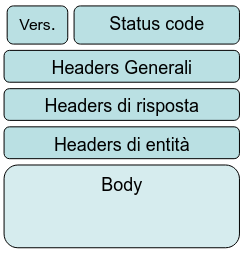
\includegraphics[width=0.3\textwidth]{img/risposta.png}
\end{center}
\begin{verbatim}
Un esempio di risposta 
GET /index.html HTTP/1.1
Host: www.cs.unibo.it:80

HTTP/1.1 200 OK
Date: Fri, 26 Nov 2007 11:46:53 GMT
Server: Apache/1.3.3 (Unix)
Last-Modified: Mon, 12 Jul 2007 12:55:37 GMT
Accept-Ranges: bytes
Content-Length: 3357
Content-Type: text/html
<HTML> …. </HTML>
\end{verbatim}
\vspace{2em} 
Vediamo ora due proprietà importanti
\begin{itemize}
  \item Sicurezza: un metodo è sicuro se non genera cambiamenti allo stato interno del server, può essere eseguito da un nodo intermedio
  \item Idempotenza: l’effetto sul server di più richieste identiche è lo stesso di quello di una sola richiesta, può essere ri-eseguito da più agenti o in più tempi diversi senza effetti negativi
\end{itemize}
\subsection*{Status code}
Lo status code è un numero di tre cifre, di cui la prima indica la classe della risposta, e le altre due la risposta specifica
\begin{itemize}
  \item 1xx: Informational (Una risposta temporanea alla richiesta, durante il suo svolgimento)
  \item 2xx: Successful (server ha ricevuto, capito e accettato la richiesta)
  \item 3xx: Redirection (La richiesta è corretta, ma sono necessarie altre azioni da parte del client per portare a termine la richiesta)
  \item 4xx: Client error (ichiesta del client non può essere soddisfatta per un errore da parte del client)
  \item 5xx: Server error (la richiesta può anche essere corretta, ma il server non riesce a soddisfarla per un problema interno)
\end{itemize}
Esempi di status code
\begin{verbatim}
100 Continue (se il client non ha ancora mandato ilbody)
200 Ok (GET con successo)
201 Created (PUT con successo)
301 Moved permanently (URL non valida, il server conosce la nuova posizione)
400 Bad request (errore sintattico nella richiesta)
401 Unauthorized (manca l’autorizzazione)
403 Forbidden (richiesta non autorizzabile)
404 Not found (URL errato)
500 Internal server error (tipicamente un errore nel codice server-side)
\end{verbatim}
\subsection*{header}
Gli header sono righe di testo (RFC822) che specificano informazioni aggiuntive
\begin{figure}[h] % [h] = qui (here)
    \centering
    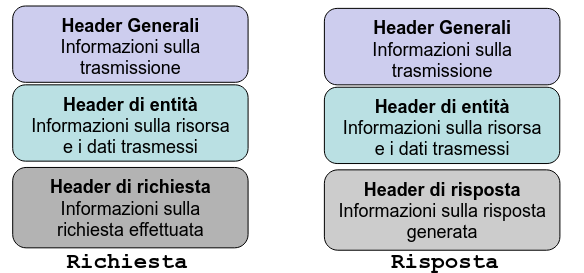
\includegraphics[width=0.5\textwidth]{img/header.png}
\end{figure} \\
\textbf{Header generali}:  si applicano solo al messaggio trasmesso e si applicano sia ad una richiesta che ad una risposta, ma non necessariamente alla risorsa trasmessa. \\
\textbf{Header dell’entità}: danno informazioni sul body del messaggio, o, se non vi è body, sulla risorsa specificata. \\
\textbf{Header della richiesta}: sono posti dal client per specificare informazioni sulla richiesta e su se stesso al server. \\
\textbf{Header della risposta}: sono posti dal client per specificare informazioni sulla risposta e su se stesso al client. \\
\subsection*{API REST}
Un API Web descrive un'interfaccia HTTP che permette ad applicazioni remote di utilizzare i servizi di dell'applicazione
\subsection{REST}
Acronimo di REpresentional State Transfer, ed è il modello architetturale che sta dietro al World Wide Web e in generale dietro alle applicazioni web "ben fatte" secondo i progettisti di HTTP. \\
Un’applicazione REST si basa fondamentalmente sull’uso dei protocolli di trasporto (HTTP) e di naming (URI) per generareinterfacce generiche di interazione con l’applicazione, e fortemente connesse con l’ambiente d’uso.
\begin{center}
L’obiettivo è creare API consistenti, predicibili e facili da capire e usare
\end{center}
L'architettura si basa su:
\begin{itemize}
  \item Definire \textbf{risorsa} ogni concetto rilevante dell’applicazione Web
  \item Associargli un \textbf{URI} come \textbf{l’identificatore} e selettore primario
  \item Usare i verbi HTTP per esprimere ogni \textbf{operazioni} dell’applicazione secondo il modello CRUD
  \begin{itemize}
    \item Creazione di un nuovo oggetto (metodo PUT)
    \item Visualizzazione dello stato della risorsa (metodo GET)
    \item Cambio di stato della risorsa (metodo POST)
    \item Cancellazione di una risorsa (metodo DELETE)
  \end{itemize}
  \item Esprimere in maniera parametrica ogni \textbf{rappresentazione dello stato interno della risorsa}, personalizzabile dal richiedente attraverso un \textbf{Content Type} preciso
\end{itemize}
\textbf{Descrivere una RESTful API}: Una API è RESTful se utilizza i principi REST nel fornire accesso ai servizi che offre
\begin{itemize}
  \item end-point (URI / route) che supporta separando collezioni e elementi singoli
  \item metodi HTTP di accesso GET, PUT, POST, DELETE
  \item rappresentazioni in \textit{Input} e \textit{Output}
  \item condizioni di errore e i messaggi che restituisce in questi casi
\end{itemize}
\subsection*{Il modello CRUD}
Pattern tipico delle applicazioni di trattamento dei dati
\begin{itemize}
  \item Create: inserimento nel database di un nuovo record
  \item Read: accesso in lettura al database
  \item Update
  \item Delete
\end{itemize}
\section{Introduzione a Javascript}
Nato nel 1995 con il nome di JavaScript (prima ECMAScript) introdotto da Sun e Netscape. Standardizzato da ECMA International nel 1997. Per 18 anni sono state fatte piccole estensioni e modifiche. Nel giugno 2015 è stata approvata la versione 6  sono state introdotte molte differenze, molti nuovi costrutti.
\textbf{Come eseguire uno script?}
\begin{itemize}
  \item Client-side: eventi
  \begin{itemize}
    \item Ogni elemento del documento ha alcuni eventi associati (click, mouseover, doppio click, tasto di tastiera, ecc), e degli attributi on+evento associati.
    \item inserendo istruzioni JavaScript (o chiamata a funzione) nel valore dell'attributo si crea una chiamata callback.
  \end{itemize}
  \item Server-side: routing
  \begin{itemize}
    \item I servizi server-side sono associati a URI. Il modo più antico e semplice è creare servizi diversi e inserirli in file separati, ciascuno con un URI proprio. Aprendo una connessione all'URI, viene invocato lo script ed eseguito il servizio.
  \end{itemize}
\end{itemize}
\textbf{Come eseguire uno script su browser?}
\begin{itemize}
  \item In maniera sincrona, appena lo script viene letto, in un tag <script> o in un file
  \item In maniera asincrona, associando il codice ad un evento sul documento (e.g., il click su un bottone): event-oriented processing
  \item In maniera asincrona, associando il codice al completamento di un’operazione di rete.
  \item In maniera asincrona, associando il codice ad un timeout, i.e., un periodo di attesa dopo il quale lo script viene eseguito automaticamente
\end{itemize}
Durante l’esecuzione dello script, il browser è bloccato e non reagisce agli input dell’utente.  \\
\vspace{1em}
\textbf{Come vediamo gli output?}
\begin{itemize}
  \item \textit{document.write(string);} (scrivendo direttamente nella finestra del browser)
  \item \textit{console.log(string);} (scrivendo sulla console)
  \item \textit{alert(string);} (scrivendo in una finestra di alert)
  \item \textit{document.getElementById(id).innerHTML = string;} (modificando il DOM del documento visualizzato)
\end{itemize}
\vspace{1em}   
\subsection{Tipi di dato}
JavaScript è minimale e flessibile per quel che riguarda i tipi di dati
\begin{itemize}
  \item booleani
  \item numeri (interi e floating)
  \item stringhe
  \item null
  \item undefined
  \item \textit{object} (unico tipo di dato strutturato, anche gli array ne fanno parte)
  \begin{itemize}
    \item Gli object sono liste non ordinate di proprietà, coppie nome-valore.
    \begin{lstlisting}
    let persona = {
      nome: 'Giuseppe',
      cognome: 'Rossi',
      altezza: 180,
      nascita: new Date(1995,3,12)
    }
\end{lstlisting}
  \end{itemize}
\end{itemize}
\subsection{Oggetti Predefiniti}
JavaScript predefinisce alcuni oggetti utili per raccogliere insieme i metodi più appropriati per certi tipi di dati.
\begin{itemize}
  \item Oggeti multipli
  \begin{itemize}
    \item Object
    \item Array
    \item String
    \item Date
    \item Number 
    \item RegExp
    \item $\vdots$
  \end{itemize}
  \item Oggetti singleton
  \begin{itemize}
    \item Math
    \item Json
    \item $\vdots$
  \end{itemize}
\end{itemize}
\subsection{Json}
JSON (JavaScript Object Notation) è un formato dati derivato dalla notazione usata da JS per gli oggetti.
\begin{lstlisting}
{
  "nome": ["Giuseppe", "Andrea", "Federico"],
  "cognome": "Rossi",
  "altezza": 180,
  "nascita": "1995-04-11T22:00:00.000Z",
  "indirizzo": {
    "via": {
    "strada": "Via Indipendenza",
    "numero": "15"
  },
  "citta": "Bologna",
  "nazione": "Italia"
  },
  "telefono": [
    { "tipo": "casa", "numero": "051 123456"},
    { "tipo": "cell", "numero": "335 987654"}
  ]
}
\end{lstlisting}
Tutti i linguaggi di programmazione più importanti oggi accettano e scrivono dati in JSON.
\vspace{1em} \\
\subsection{Javascript client-side}
\begin{center}
    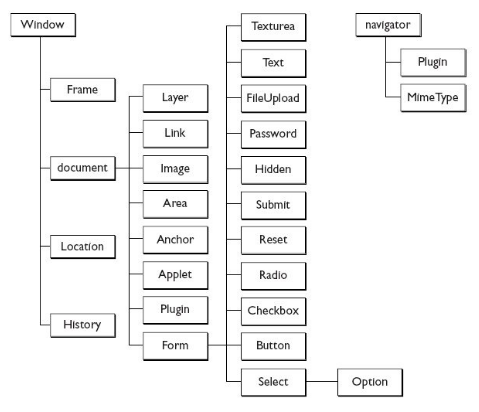
\includegraphics[width=0.5\textwidth]{img/oggetti.png}
\end{center} 
\begin{itemize}
  \item \textbf{window}:
  \begin{itemize}
    \item l’oggetto top-level con le proprietà e i metodi della finestra principale:
    \begin{itemize}
      \item posizione:moveBy(x,y), moveTo(x,y), etc.
      \item dimensioni: resizeBy(x,y), resizeTo(x,y), etc.
      \item altre finestre: open("URLname","Windowname",["opt"])
    \end{itemize}
  \end{itemize}
  \item \textbf{navigator:}
  \begin{itemize}
    \item ’oggetto con le proprietà del client come nome, numero di versione, plug-in installati, supporto per i cookie, etc.
  \end{itemize}
  \item \textbf{location}
  \begin{itemize}
    \item ’URL del documento corrente. Modificando questa proprietà il client accede a un nuovo URL (redirect):
    \begin{itemize}
      \item window.location ="http://www.cs.unibo.it/";
      \item window.location.href ="http://www.cs.unibo.it/";
    \end{itemize}
  \end{itemize}
  \item \textbf{history}
  \begin{itemize}
    \item 'array degli URL acceduti durante la navigazione. Possibile creare applicazioni client-side dinamiche che 'navigano la cronologia’:
    \begin{itemize}
      \item Proprietà: length, current, next
      \item Metodi: back(), forward(), go(int)
    \end{itemize}
  \end{itemize}
  \item \textbf{document}
  \begin{itemize}
    \item appresenta il contenuto del documento, ed ha proprietà e metodi per accedere ad ogni elemento nella gerarchia:
    \begin{itemize}
      \item document.title: titolo del documento
      \item document.forms[0]: il primo form
      \item document.forms[0].checkbox[0]: la prima checkbox del primo form
      \item document.forms[0].check1: l’oggetto con nome "check1" nel primo form (non per forza una checkbox!)
      \item document.myform: l’oggetto "myform"
      \item document.images[0]: la prima immagine
    \end{itemize}
    \item Inoltre document rappresenta l'oggetto DOMDocument del DOM del documento visualizzato
  \end{itemize}
\end{itemize}
\textbf{Modello di documento} \\
Ogni oggetto nella gerarchia è caratterizzato da un insieme di proprietà, metodi ed eventi che permettono di accedervi, controllarlo, modificarlo. \\
Javascript nacque per controllare i valori di un form:
\begin{lstlisting}
function verify() {
  if (document.forms[0].elements[0].value == ""){
    alert("Il nome e' obbligatorio!")
    document.forms[0].elements[0].focus();
    return false;
  }
  return true;
}
<form action= "..." onSubmit="Verify()">
<p>Name: <input type="text" name="userName"> </p>
\end{lstlisting}
\vspace{1em} 
\subsection{Il Document Object Model (DOM)}
Il Document Object Model è un interfaccia di programmazione (API) per documenti sia HTML sia XML. Definisce la struttura logica dei documenti ed il modo in cui si accede e si manipola un documento. \\
Ogni componente di un documento HTML o XML può essere \textit{letto, modificato, cancellato} o aggiunto utilizzando il Document Object Model.
\begin{center}
    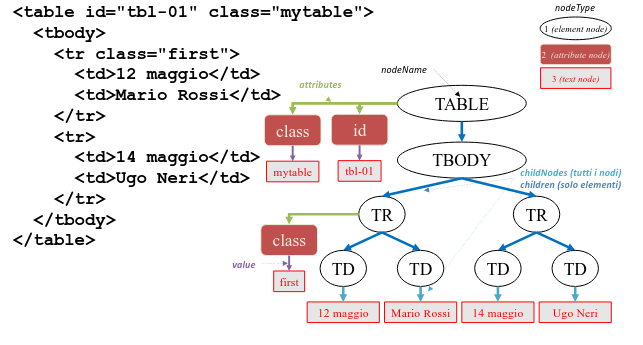
\includegraphics[width=0.8\textwidth]{img/dom.png}
\end{center} 
\subsection{Oggetti del DOM}
l core del DOM definisce alcune classi fondamentali per i documenti HTML e XML, e ne specifica proprietà e metodi. La classe principale di DOM è DOMNode, di cui la maggior parte delle altre classi è una sottoclasse. \\
Le classi principali definiti nel DOM sono:
\begin{itemize}
  \item DOMDocument : il documento di cui si sta parlando
  \item DOMElement: ogni singolo elemento del documento
  \item DOMAttr: ogni singolo attributo del documento
  \item DOMText: ogni singolo nodo di testo del documento
  \item DOMComment, DOMProcessingInstruction, DOMCDATASection, DOMDocumentType, ecc.
\end{itemize}
\subsection{DOM Node}
\textbf{DOMNode} specifica i metodi per accedere a tutti gli elementi di un nodo di un documento, inclusi il nodo radice, il nodo documento, i nodi elemento, i nodi attributo, i nodi testo, ecc. Semplificando:
\begin{center}
    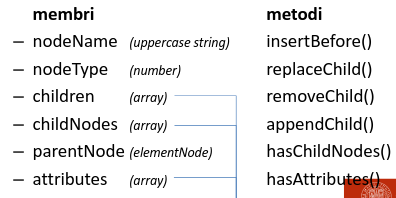
\includegraphics[width=0.6\textwidth]{img/domnode.png}
\end{center} 
\subsection{DOM Element}
DOMElement specifica i metodi e i membri per accedere a qualunque elemento del documento. Semplificando
\begin{center}
    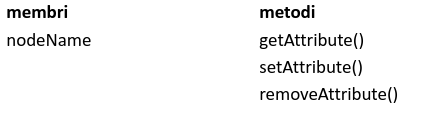
\includegraphics[width=0.6\textwidth]{img/domelement.png}
\end{center} 
e analogamente per le altre classi ed interfaccia del DOM.
\subsection*{Javascript e DOM}
Javascript implementa i metodi standard per accedere al DOM del documento.
\begin{lstlisting}
var c = document.getElementById('c35');

c.setAttribute('class','prova1');
c.removeAttribute('align') ;
var newP = document.createElement('p');
var text = document.createTextNode('Ciao Mamma.');

newP.appendChild(text);
c.appendChild(newP);
\end{lstlisting}
Creiamo una lista:
\begin{lstlisting}
// Creazione elementi singoli
Olist = document.createElement("ol");
voce1 = document.createElement("li");
voce2 = document.createElement("li");
testo1 = document.createTextNode("un po' di testo");
testo2 = document.createTextNode("altro testo - item 2");

// Creazione lista completa
voce1.appendChild(testo1);
voce2.appendChild(testo2);
Olist.appendChild(voce1);
Olist.appendChild(voce2);

// Inserimenti lista in una data posizione
div = document.getElementById("lista");
body = document.getElementsByTagName("body").item(0);
body.insertBefore(Olist,div);
\end{lstlisting}
\subsection*{innerHTML e outerHTML}
Il DOM per HTML (non generale!) permette di leggere/scrivere interi elementi, trattandoli come stringhe:
\begin{itemize}
  \item \textbf{innerHTML}: legge/scrive il contenuto di un sottoalbero (escluso il tag dell’elemento radice)
  \item \textbf{outerHTML}: legge/scrive il contenuto di un elemento (incluso il tag dell’elemento radice)
\end{itemize}
\subsection{Navigare sul DOM}
\begin{itemize}
  \item Il DOM (sia HTML sia XML) non ha metodi propri per navigare sull'albero liberamente.
  \item L'unico modo "ufficiale" è iterativamente esplorare l'albero attraverso la proprietà children.
\end{itemize}
\begin{lstlisting}
//Trova la n-esima cella della m-esima riga della tabella con id dato
function getCell(tId,row,cell) {
  let items = document.body.children;
  let i = 0;
  do while (items[i].id !== tId) { i++ } ;
  let j = 0;
  do while (items[i].children[j].nodeName !== 'TBODY') {j++}
  let rows = items[i].children[j].children
  return rows[row].children[cell]
}
\end{lstlisting}
\subsection*{Selettori base HTML in DOM}
I metodi base in DOM per accedere ai nodi di un documento sono:
\begin{itemize}
  \item \textbf{getElementById}
  \begin{itemize}
    \item solo ovviamente se l'elemento ha un id
  \end{itemize}
  \item \textbf{getElementsByName}
  \begin{itemize}
    \item se l'elemento ha un attributo name
  \end{itemize}
  \item \textbf{getElementsByTagName}
  \begin{itemize}
    \item tutti gli elementi con nome specificato
  \end{itemize}
\end{itemize}
\subsection*{Javascript ed eventi DOM}
avascript permette di associare callback di eventi ad oggetti (dichiarazione locale o globale)
\begin{lstlisting}
<script language="JavaScript">
  window.onkeypress= pressed;
  window.document.onclick = clicked;

  function pressed(e) { alert("Key pressed: " + e.which);}
  function clicked() { alert("Mouse Click! "); }
</script>
...
<body>
  <p id="mypara">Puoi
    <a href="test.htm" onClick="alert('Link!');">
      cliccare qui
    </a>
    oppure qui.
  </p>
</body>
\end{lstlisting} 
\vspace{1em}
Tutta la parte di sintassi/logica di JS non la riscrivo, la trovi in \textit{18-Javascript-3.pdf}. \\
\section{Approfondimenti su HTTP}
\begin{center}
    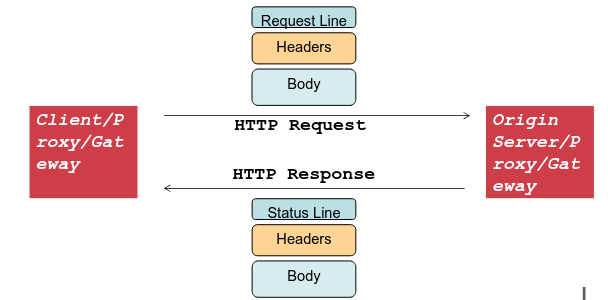
\includegraphics[width=0.6\textwidth]{img/recap.png}
\end{center} 
\subsection{HTTP/2}
Inizialmente chiamato HTTP 2.0 è la seconda major revision di HTTP.Non è una riscrittura del protocollo, i concetti principali e la compatibilità con HTTP 1.x restano: metodi, status code, headers, etc. Inizialmente proposto nel 2012 e standardizzato da IETF nel RFC 7540 a Maggio 2015 (HTTP1.1 è del 1997!).
\begin{itemize}
  \item HTTP/2 ha introdotto importanti novità mirate a migliorare le \textbf{performance}, tra cui:
  \begin{itemize}
    \item \textbf{multiplexing}: nella stessa connessione è possibile avere richieste e risposte multiple, restituite anche in ordine diverso rispetto alle richieste e “ricostruite” nel client
    \item supporto per operazioni di \textbf{Push}: il server può spedire più dati al client di quelli richiesti anticipando richieste successive nella stessa connessione
  \end{itemize}
  \begin{center}
    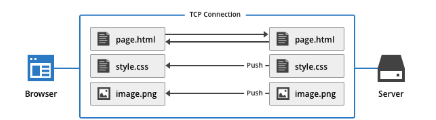
\includegraphics[width=0.6\textwidth]{img/push.png}
\end{center} 
\end{itemize}
Concettualmente HTTP/2 è identico ad HTTP 1.1: ruoli, verbi, headers sono gli stessi. Tuttavia è un protocollo binario in cui i messaggi non sono più plaintext, ma codificati in maniera \textbf{compressa} e separando il blocco degli header dal payload. Ogni flusso di dati (stream) è suddiviso in frame separati e identificati che viaggiano anche sovrapposti (multiplexing).
  \begin{center}
    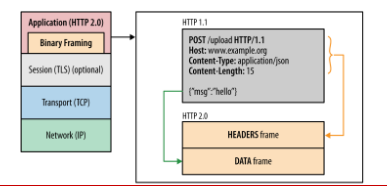
\includegraphics[width=0.6\textwidth]{img/flusso.png}
\end{center} 
L'algoritmo di compressione degli header HTTP/2 si chiama HPACK (RFC 7541). Solo gli header diversi da quelli delle richieste precedenti vengono inseriti nel frame e spediti. Secondo calcoli fatti, la compressione degli header ne riduce la dimensione del 30\%.
  \begin{center}
    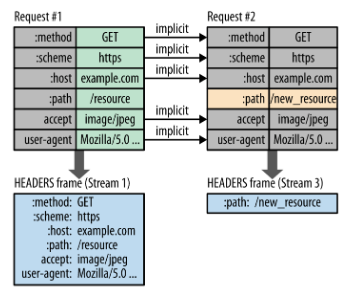
\includegraphics[width=0.4\textwidth]{img/compressione.png}
\end{center} 
\subsection{HTTP/3}
HTTP/3 è la versione più recente di HTTP, standardizzata nel 2023 come RFC 9114. L'obiettivo principale è aumentare ulteriormente le performance rispetto ad HTTP/2. Si basa sul protocollo QUIC proposto da Google nel 2012 e costruito su UDP (User Datagram Protocol), protocollo alternativo a TCP/IP. QUIC lavora a livello di trasporto e non di applicazione come HTTP. \\
HTTP/3 quindi non si basa su TCP/IP, a differenza delle precedenti versioni, ma mantiene retrocompatibilità: metodi, header, status code restano invariati
\subsection{Cookies}
HTTP è \textbf{stateless}: non esiste nessuna struttura ulteriore alla connessione e il server non è tenuto a mantenere informazioni su connessioni precedenti. 
\begin{itemize}
  \item Un cookie (\textit{concetualmente}) è una breve informazione scambiata tra il server ed il client
\end{itemize}
Il client mantiene alcune informazioni sulle connessioni precedenti, e le manda al server di pertinenza ogni volta che richiede una risorsa.
  \begin{center}
    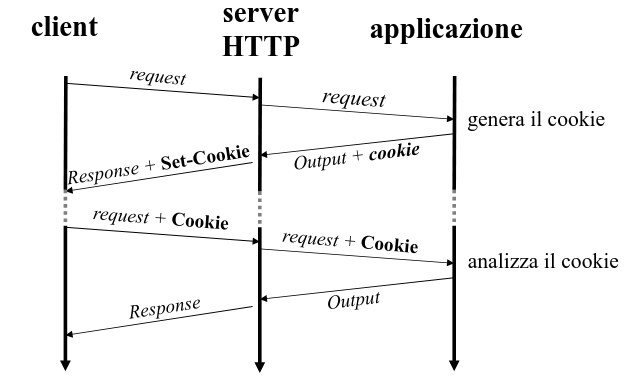
\includegraphics[width=0.6\textwidth]{img/cookies.png}
\end{center} 
\begin{itemize}
  \item Alla prima richiesta di uno user-agent, il server fornisce la risposta ed un header aggiuntivo, il cookie, con \textbf{dati arbitrari}, e con la specifica di usarlo per ogni successiva richiesta.
  \item Il server associa a questi dati ad informazioni sulla transazione.
  \item Ogni volta che lo user-agent accederà a questo sito, rifornirà i dati opachi del cookie che permettono al server di ri-identificare il richiedente
\end{itemize}
I cookies dunque usano due header, uno per la risposta, ed uno per le richieste successive:
\begin{itemize}
  \item \textbf{Set-Cookie}: header della risposta, spedito dal server, il client può memorizzarlo e rispedirlo alla prossima richiesta.
  \item \textbf{Cookie}: header della richiesta. Il client decide se spedirlo sulla base del nome del documento, dell’indirizzo IP del server, e dell’età del cookie.
\end{itemize}
\subsection{Headers e struttura dei cookie}
I cookies contengono dati arbitrari in formato testuale:
\begin{lstlisting}
  set-cookie:AWSALB=oJW4vtjxMz8WLY3jSrCUNekkG1aLZQHmblSvExmvR6agqb+f+fC4RQWCb+gLVijpRakI8RrnfrXqiDmQ9KwqA8LiVMdhkBRUCCtOgwx5JBxKLmIBQ7gnbIFIzo+; Expires=Wed, 01 May 2000 11:07:46GMT; Path=/
\end{lstlisting}
Oltre a nome e valore, includono informazioni che il client usa quando ri-spedisce il cookie:
\begin{itemize}
  \item \textbf{Domain}: il dominio per cui il cookie è valido
  \item \textbf{Path}: l'URI per cui il cookie è valido
  \item \textbf{Max-Age/Expire}: La durata in secondi del cookie
  \item \textbf{Secure}: la richiesta che il client contatti il server usando soltanto un meccanismo sicuro (es. HTTPS) per spedirlo
  \item \textbf{Version}: La versione della specifica a cui il cookie aderisce.
\end{itemize}
\subsection*{Uso dei cookie}
Esitono vari tipi di cookie usati per scopi diversi, tra cui:
\begin{itemize}
  \item \textbf{Cookie persistenti}: hanno una validità temporale lunga, o addirittura non scadono mai, e sono usati per mantenere informazioni (semi)permanenti ad esempio informazioni su login, preferenze degli utenti, ecc.
  \item \textbf{Cookie di sessione}: hanno una durata breve e sono usati per raggruppare operazioni in sessioni di lavoro; contengono un identificativo della sessione le cui informazioni sono sul server; solitamente sono cancellati alla chiusura del browser
  \begin{itemize}
    \item Autenticazione: processo di verifica dell'identità di un utente
    \begin{itemize}
      \item Session-based: il server memorizza un ID di sessione e informazioni sull'utente verificate ad ogni richiesta
      \item Token-based: il client memorizza un token, ricevuto dal server, che spedisce ad ogni richiesta ed è usato per la verifica
    \end{itemize}
    \item Autorizzazione: processo di verifica dell'effettiva possibilità di un utente di eseguire un'operazione e/o accedere a una risorsa
  \end{itemize}
  \item \textbf{Cookie di terze parti}: appartengono ad un dominio diverso rispetto a quello della pagina in cui sono caricati; usati ad esempio per banner pubblicitari, permettono di ricostruire la navigazione degli utenti e possono essere usati in modo improprio; le impostazioni dei browser permettono infatti di disabilitarli
\end{itemize}
\textbf{Header WWW-Authenticate} \\
Quando l'utente prova ad eseguire un'azione che richiede autenticazione, il server risponde con uno status code \textbf{401} (Unauthorized) e aggiunge un header \textit{WWW-Authenticate} in cui specifica i criteri da usare per l'autenticazione \\
Gli schemi più comuni:
\begin{itemize}
  \item Basic (disuso): prevede la spedizione delle informazioni di autorizzazione in chiaro ad ogni risposta
  \item Diges: Il client spedisce nell'header Authorization una fingerprint della password, ovvero la password crittografata con il metodo MD5 (RFC 1321).
  \item Bearer (usato anche per autenticazione token-based): Nello schema Bearer (RFC 6750) il client non spedisce la password, in chiaro o cifrata, ma un token ("bearer token") che gli permette di accedere ad una risorsa
\end{itemize}
  \begin{center}
    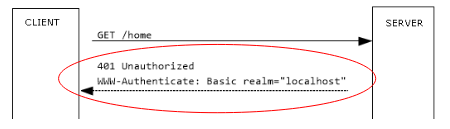
\includegraphics[width=0.6\textwidth]{img/auth.png}
\end{center} 
\subsection{Cookie di sessione}
I cookie di sessione contengono un ID univoco di sessione che il server ha memorizzato e riconosce. Il server si occupa anche di gestire la data di expiry (scadenza) del cookie e quindi chiusura della sessione.
  \begin{center}
    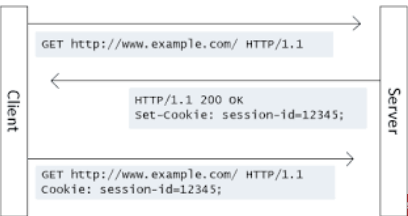
\includegraphics[width=0.4\textwidth]{img/sessione.png}
\end{center} 
Esempio in php:
  \begin{center}
    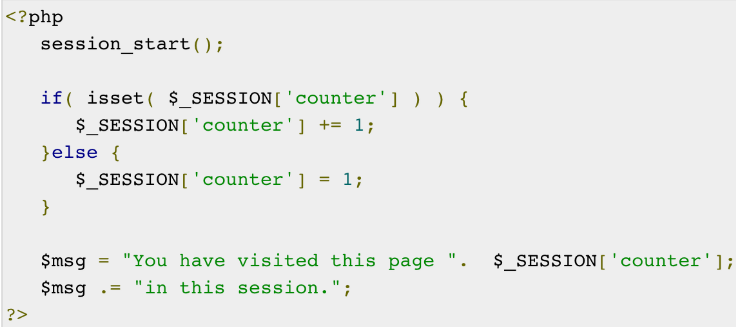
\includegraphics[width=0.6\textwidth]{img/php.png}
\end{center}
Esempio in Express.js:
  \begin{center}
    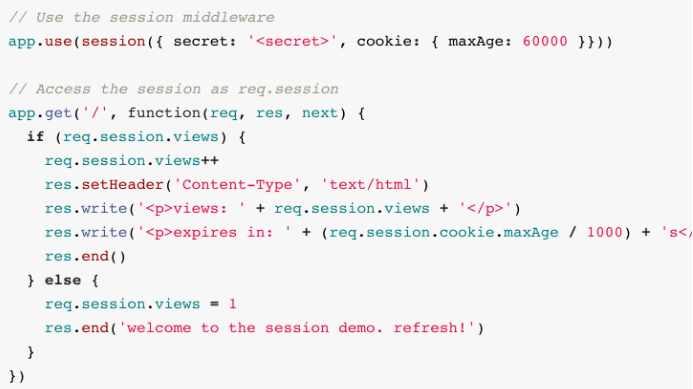
\includegraphics[width=0.8\textwidth]{img/express.png}
\end{center}
\subsection{Base 64}
Viene identificato un sottoinsieme di 64 caratteri di US-ASCII sicuri, che hanno la stessa codifica in tutte le versioni di ISO 646. \\
Ogni flusso di dati viene suddiviso in blocchi di 24 bit (3 byte). A loro volta questi 24 bit sono suddivisi in 4 blocchi di 6 bit ciascuno e codificati secondo una tabella prefissata in uno dei 64 caratteri. \\
La decodifica di Base64 è algoritmica, banale, non usa chiavi né calcoli di particolari complessità. NON È una tecnica crittografica! \\
  \begin{center}
    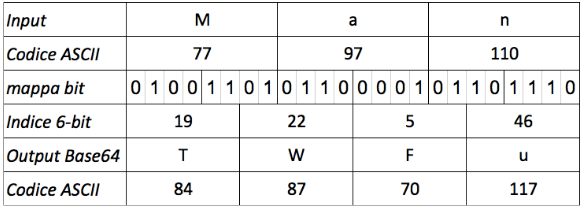
\includegraphics[width=0.6\textwidth]{img/base64.png}
\end{center}
\subsection{Header e Payload}
\begin{itemize}
  \item \textbf{Header}: specifica il tipo di token e l'algoritmo di cifratura utilizzato
  \item \textbf{Payload}: informazioni di interscambio organizzate in affermazioni (claims) che possono essere di tre tipi:
  \begin{itemize}
    \item Registered: claim predefiniti utili per descrivere il token
    \item Public: arbitrari ma dichiarati nello IANA JSON Web Token Registry per evitare conflitti
    \item Private: arbitrari e personalizzabili, utili per scambiare dati tra applicazioni che si accordano sui dati da usare
  \end{itemize}
\end{itemize}
\subsection{Signature}
Il token (header e payload, in base64) può essere firmato con una chiave segreta lato server in modo da poterlo verificare nelle successive richieste e, se corrotto, non considerarlo valido.  Cifratura simmetrica e asimmetrica (es. SHA256). \textbf{Il contenuto del token non è cifrato ma solo codificato in base64!} Si può decodificare facilmente, non bisogna quindi inserire dati sensibili. \\
\vspace{1em} \\
\subsection{CORS}
Supponiamo che in una pagina appartenente ad un dominio protetto (es. in una sessione autenticata) si riesca ad intrufolare un pezzo di codice malizioso, che raccoglie e trasmette informazioni ad un repository accessibile ai malintenzionati.
\begin{itemize}
  \item Si parla di vulnerabilità tra domini o \textbf{cross-domain}
\end{itemize}
Una delle possibili soluzioni, chiamata CORS, si basa sull'uso del metodo OPTION per indicare i domini ammessi.
  \begin{center}
    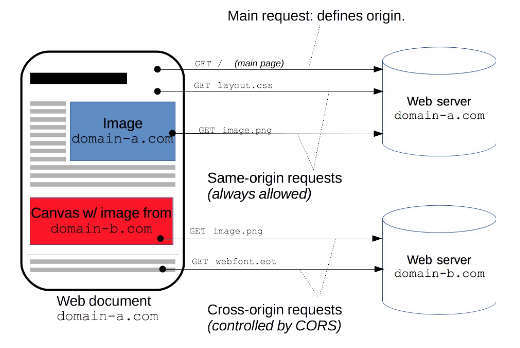
\includegraphics[width=0.6\textwidth]{img/cors.png}
\end{center}
\textbf{Cross-Origin Resource Sharing}: Una tecnica tutta HTTP introdotta dal W3C (W3C Rec 29/1/2013). \\
Si attiva solo per le connessioni Ajax (non si usa per connessioni HTTP normali) e prevede l'uso di due nuovi header:
\begin{itemize}
  \item nella richiesta: \textbf{Origin}, per specificare il dominio su cui si trova il contenuto
  \item nella risposta: \textbf{Access-Control-Allow-Origin} per indicare gli altri domini da cui è permesso caricare contenuti
\end{itemize}
\subsection{HTTP Caching}
HTTP offre sofisticati meccanismi di caching, molto utili in applicazioni RESTFUL. Può essere client-side, server-side o su un proxy (intermedia). \\
La cache server-side riduce i tempi di computazione di una risposta, ma non ha effetti sul carico di rete, le altre riducono il carico di rete. \\
HTTP 1.1 introduce due tipi di meccanismi per controllare la validità dei dati in cache (cache control):
\begin{itemize}
  \item Server-specified expiration
  \begin{itemize}
    \item Il server indica una scadenza della risorsa. Può usare due meccanismi: header Expires o direttiva max-age in Cache-Control.
    \item Se la data di scadenza è già passata, la richiesta deve essere rivalidata.
  \end{itemize}
  \item Heuristic expiration
  \begin{itemize}
    \item Poiché molte pagine non conterranno valori espliciti di scadenza, la cache stabilisce valori euristici di durata delle risorse, dopo le quali assume che sia scaduta. Usa informazioni contenute in altri header, ad esempio \textit{Last-Modified time}
    \item L'algoritmo esatto non è fissato nelle specifiche di HTTP ma dipende dall'implementazione
  \end{itemize}
\end{itemize}
\section{}
\end{document} 


